\subsection{External Interface Requirements}
	\subsubsection{User Interfaces}
		Here we provide some basic mockups to show how the interface should appear to the user:\newline
		
		\begin{figure}[H]	
			\centerline{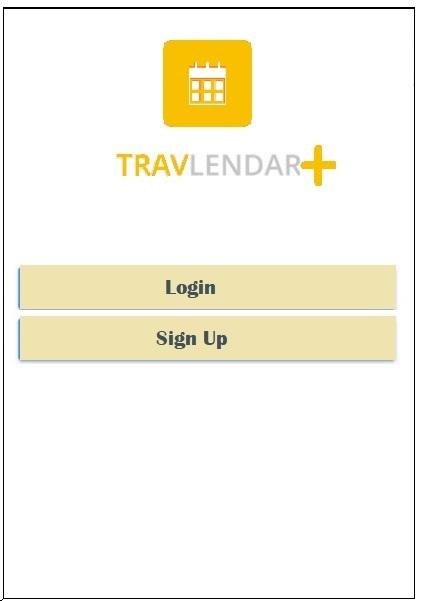
\includegraphics[scale=0.4]{Images/Login}}
			\caption{Login}
		\end{figure}	
		\begin{figure}[H]		
			\centerline{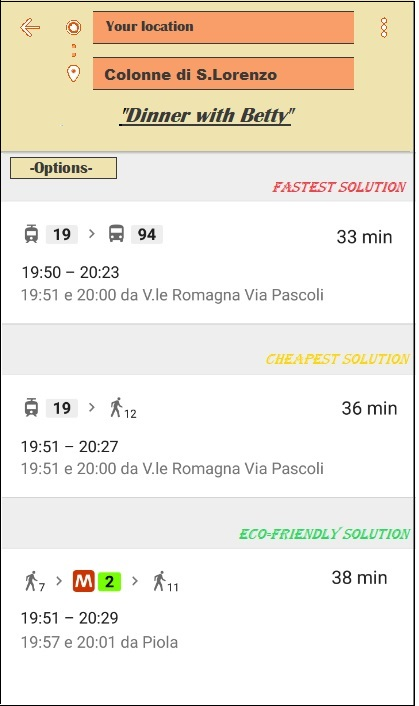
\includegraphics[scale=0.4]{Images/suggestedsolution}}
			\caption{Select solution}
		\end{figure}	
		\begin{figure}[H]
			\centerline{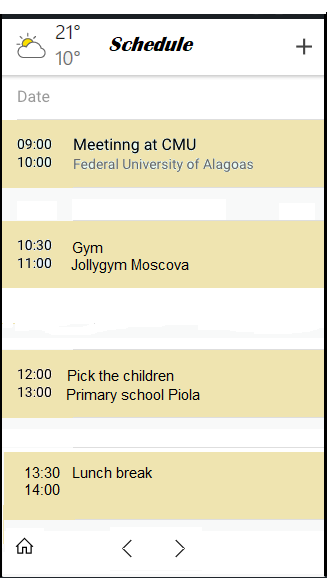
\includegraphics[scale=0.5]{Images/schedule}}
			\caption{Visualize schedule}
		\end{figure}
	
	\subsubsection{Hardware Interfaces}
	The main hardware interface of the system consists in the access to the GPS data
	in the mobile application. The application also requires Internet connectivity
	and internal storage access.
	
	\subsubsection{Software Interfaces}
	The mobile application must support Android, iOS and the remaining main OSs (further details are discussed in paragraph 3.6.5 Portability). The web application
	works on any web server that supports Java. The back-end stores its data in a
	DBMS and can run on every platform that supports the JVM.
	\subsubsection{Communication Interfaces}
	The communication between clients and server should be HTTP requests/responses based.
\subsection{UML modeling}
	In this section, we formalize the S2B in terms of UML models.\newline
	We divided the Use Case Diagrams into parts to slightly improve the readability of the Diagrams. After the Diagrams, descriptions of the main Use Cases are provided.\newline
	After that we provide a Class Diagram of the whole system and then some Activity Diagrams, to better explain the structure of the S2B and its behavior.\newline
	Other types of diagrams have been considered, but we eventually realized them to not provide, at this stage, any other notable information about the system.
	\subsubsection{Use Case diagram}
		\smallskip
		\begin{figure}[H]	
			\centerline{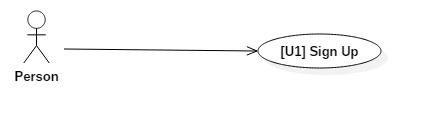
\includegraphics[scale= 0.7]{Images/UseCaseDiagram0}}
			\caption{Person Use Case Diagram}
		\end{figure}
		\begin{figure}[H]	
			\centerline{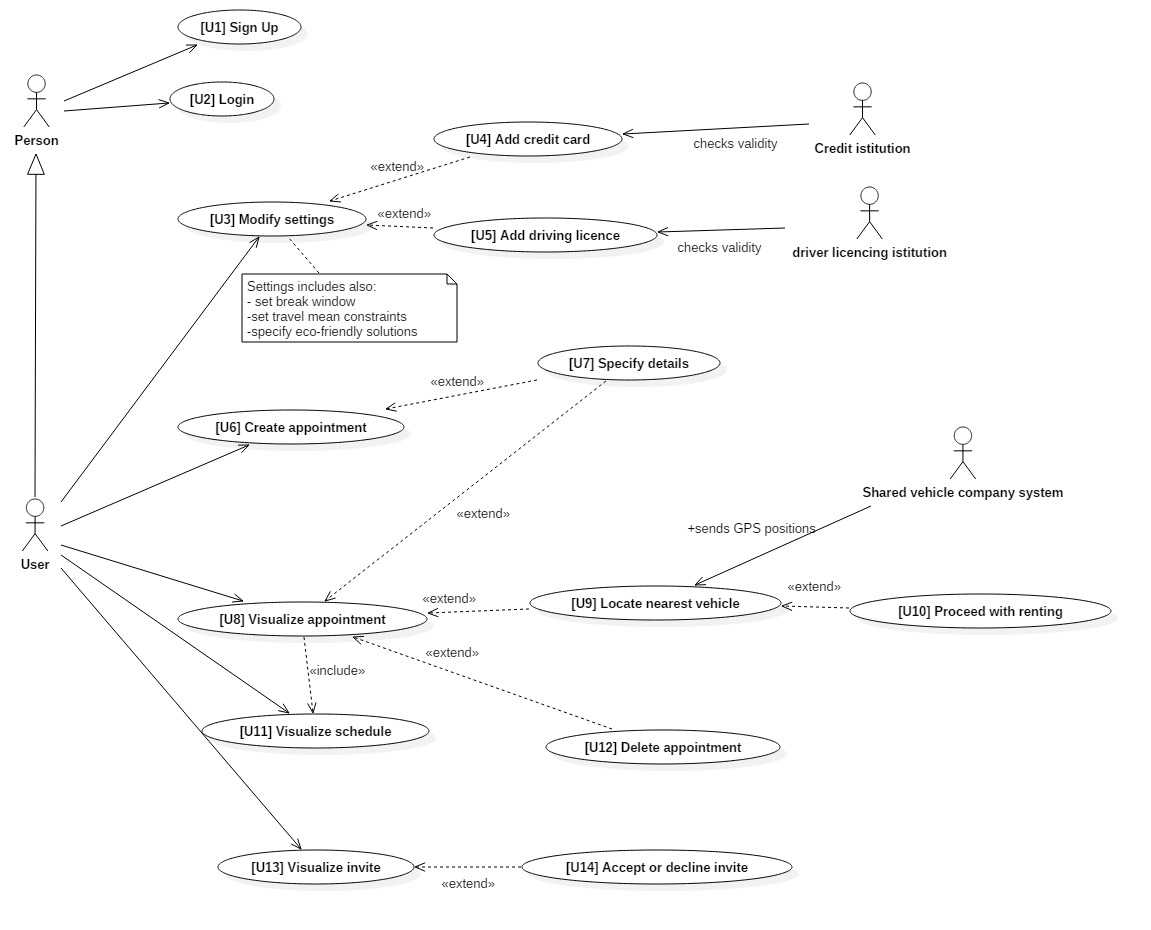
\includegraphics[width=\paperwidth-1]{Images/UseCaseDiagram1}}
			\caption{User Use Case Diagram}
		\end{figure}

	\begin{figure}[H]	
	\centerline{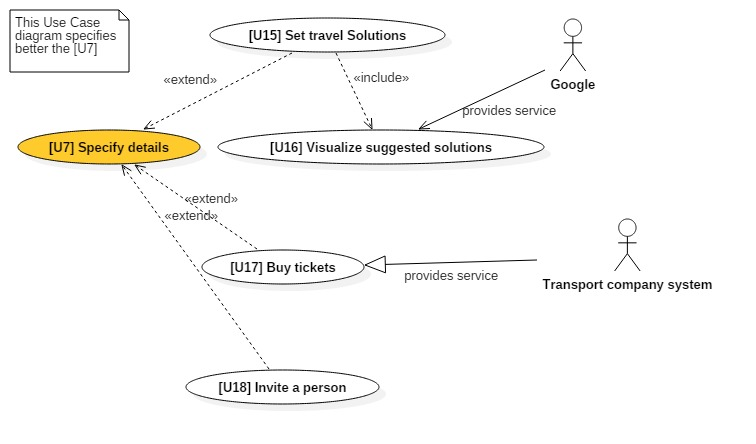
\includegraphics[width=\paperwidth-1]{Images/UseCaseDiagram2}}
	\caption{ "Specify Details" Use Case }
\end{figure}
		\renewcommand{\arraystretch}{1.6} % increase line height
		
		\medskip %leave a bit of space before the next 'section'
		\vbox{ % to avoid page breaking
			\noindent
			\textbf{User creates appointment}
			\medskip\\
			\begin{tabu} to \textwidth {| X[\fcWidth,r,p] | X[1-\fcWidth,l,p] |}
				\hline\textbf{Use case:} & User creates an appointment
				\\
				\hline\textbf{Actors:} & User
				\\
				\hline\textbf{Entry condition:} & The user must be logged
				\\
				\hline\textbf{Flow of events:} & The user creates an appointment giving it a name;\newline
				User specifies the time and date of the appointment;\newline
				User specifies the location of the appointment;\newline
				User specifies the type of the appointment;\newline
				User specifies details such as passengers or baggage;\newline
				User selects a travel mean taking into account app's suggestions;\newline
				The app takes note of the settings and send a confirmation;\newline
				The app redirects the User to the main page.
				\\
				\hline\textbf{Secondary flows:} & User does not specify a travel mean and let it blank;\newline
				The app takes anyway note of the setting and alert the user of the missing information; \newline
				The app redirects the user to the main page.
				\\
				\hline\textbf{Exceptions:} & Warnings messages are created in the following cases:
				\begin{itemize}
					\item User creates an appointment that overlaps with another appointment;
					\item User creates an appointment with a location that is unreachable in the allocated time;
					\item User creates an appointment that violates the set constraints about the break windows.
				\end{itemize}
				\\
				\hline\textbf{Post conditions:} & The user is successfully redirected to the main page.
				\\
				\hline
   			\end{tabu}
			\bigskip %leave a bit of space after the table
		}
		
		\vbox{ % to avoid page breaking
			\noindent
			\textbf{Sign Up}
			\medskip\\
			\begin{tabu} to \textwidth {| X[\fcWidth,r,p] | X[1-\fcWidth,l,p] |}
				\hline\textbf{Use case:} & Sign Up
				\\
				\hline\textbf{Actors:} & Person
				\\
				\hline\textbf{Entry condition:} &none;
				\\
				\hline\textbf{Flow of events:} & the Person inserts \defined{valid credentials};\newline
				the app sends an email with the confirmation link;\newline
				the Person gives the confirmation through the link on the mail;\newline
				the app shows the \defined{welcome page} to the new User.
				
				\\
				\hline\textbf{Secondary flows:} & none.
				\\
				\hline\textbf{Exceptions:} &the person inserts non \defined{valid credentials};\newline
				the sign-up cannot proceed.
				
				\\
				\hline\textbf{Post conditions:} & the person is successfully signed up and become an actual User.
				\\
				\hline
			\end{tabu}
			\bigskip %leave a bit of space after the table
		}
		
		\vbox{ % to avoid page breaking
			\noindent
			\textbf{Initial settings configuration}
			\medskip\\
			\begin{tabu} to \textwidth {| X[\fcWidth,r,p] | X[1-\fcWidth,l,p] |}
				\hline\textbf{Use case:} & Initial settings configuration
				\\
				\hline\textbf{Actors:} & User
				\\
				\hline\textbf{Entry condition:} & the User has just completed the sign up process;\newline
				User must be logged.
				
				\\
				\hline\textbf{Flow of events:} & User inserts sequentially the following  information:
				\begin{itemize}
				\item 	Credit card;
				\item 	Break time windows;
				\item	Interest for Eco-friendly solutions on the travel means.
				\item	Constraints on travel means.
				\end{itemize}
				The app, for each step,  checks the info and sends a confirmation;
				The app redirects the User to the main page.
				
				\\
				\hline\textbf{Secondary flows:} & User skips specifying one or more information that could be specified later in the settings.\newline
				The app notifies the user about the missing information and redirects anyway the user to the main page.
				
				\\
				\hline\textbf{Exceptions:} & user inserts inconsistent information (incorrect credit-card information, break time shorter than 30 minutes);\newline
				The app alerts the user and asks him to insert again the info.
				\\
				\hline\textbf{Post conditions:} & the set \defined{preferences} are successfully saved and the user is redirected to the main page.
				\\
				\hline
			\end{tabu}
			\bigskip %leave a bit of space after the table
		}
		
		\vbox{ % to avoid page breaking
			\noindent
			\textbf{User specifies the appointment}
			\medskip\\
			\begin{tabu} to \textwidth {| X[\fcWidth,r,p] | X[1-\fcWidth,l,p] |}
				\hline\textbf{Use case:} & User specifies appointment's details.
				\\
				\hline\textbf{Actors:} & User
				\\
				\hline\textbf{Entry condition:} & User must be logged;\newline
				the appointment must exist;
				
				\\
				\hline\textbf{Description:} & User specifies or modifies basic details (time, date, location, type of appointment, number of passengers and the presence of baggage) and eventually:
				\begin{itemize}
					\item If not specified yet, sets a transportation mean;
					\item Modifies the previous transportation mean;
					\item Buys a ticket for the transportation mean;
					\item Invites a person. 
				\end{itemize}\\
				\hline
			\end{tabu}\\
			\bigskip %leave a bit of space after the table
		}
		
		\vbox{ % to avoid page breaking
			\noindent
			\textbf{User buy travel ticket}
			\medskip\\
			\begin{tabu} to \textwidth {| X[\fcWidth,r,p] | X[1-\fcWidth,l,p] |}
				\hline\textbf{Use case:} & User buys travel ticket
				\\
				\hline\textbf{Actors:} & User
				\\
				\hline\textbf{Entry condition:} & User must be logged; \newline
				User must have added a payment card.
				
				\\
				\hline\textbf{Flow of events:} & User selects an appointment;\newline
				User,  through the app, searches for tickets for the specified transportation mean; \newline
				User selects the ticket’s option and picks one;\newline
				User proceeds with the payment;\newline
				The payment operation ends successfully;\newline
				The app sends a confirmation and redirects the User to the main page;
				
				\\
				\hline\textbf{Secondary flows:} & none
				\\
				\hline\textbf{Exceptions:} & The payment is rejected (not enough credit, expired card, ..);\newline
				The app notifies the User; \newline
				The app redirects the User to the main page;
				
				\\
				\hline\textbf{Post conditions:} & User successfully books the tickets and is redirected to the main page.
				\\
				\hline
			\end{tabu}
		}
	\subsubsection{Class diagram}
		% don't really know what happens here, but it is fine graphically
		% ((I'm referring to '\paperwidth-1')
		\begin{figure}[H]
			\centerline{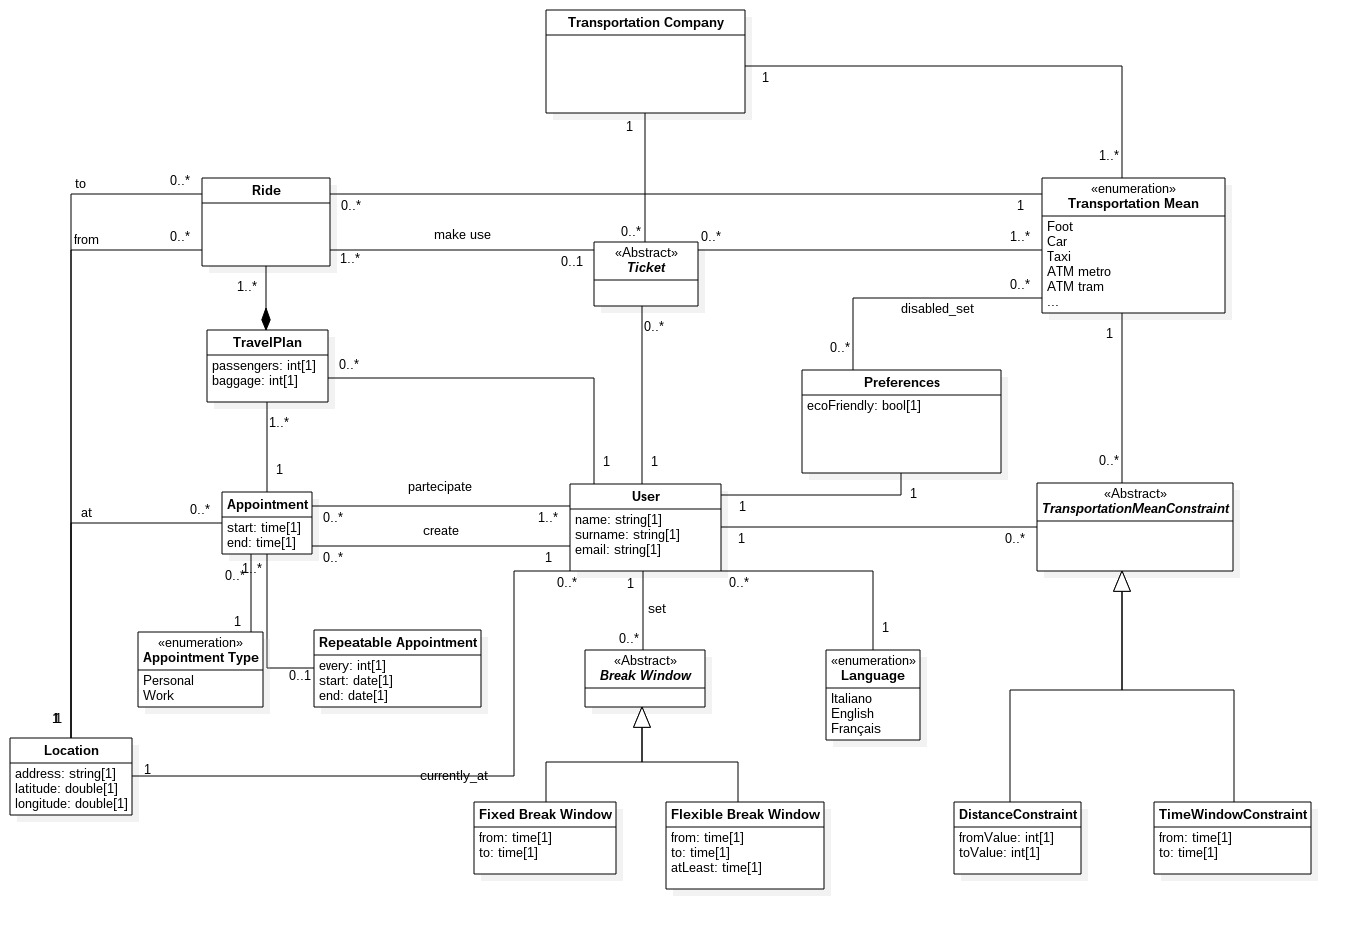
\includegraphics[width=\paperwidth-1]{Images/ClassDiagram}}
			\caption{General Class Diagram}
		\end{figure}
	\subsubsection{Activity diagrams}
		\begin{figure}[H]
			\centerline{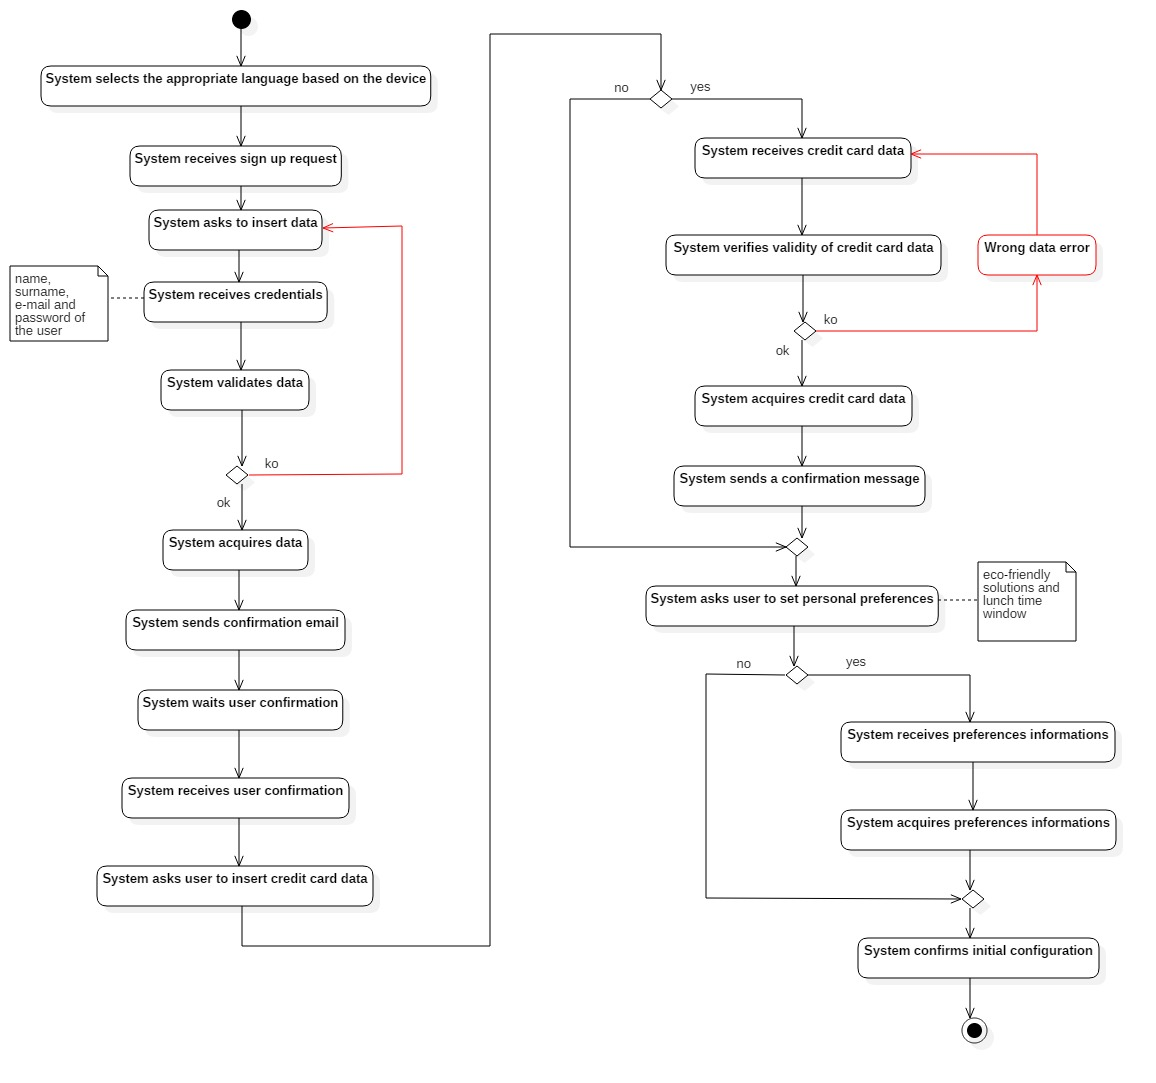
\includegraphics[width=\paperwidth-1]{Images/RegistrationDiagramAD}}
			\caption{Registration Activity Diagram}
		\end{figure}
		\begin{figure}[H]
			\centerline{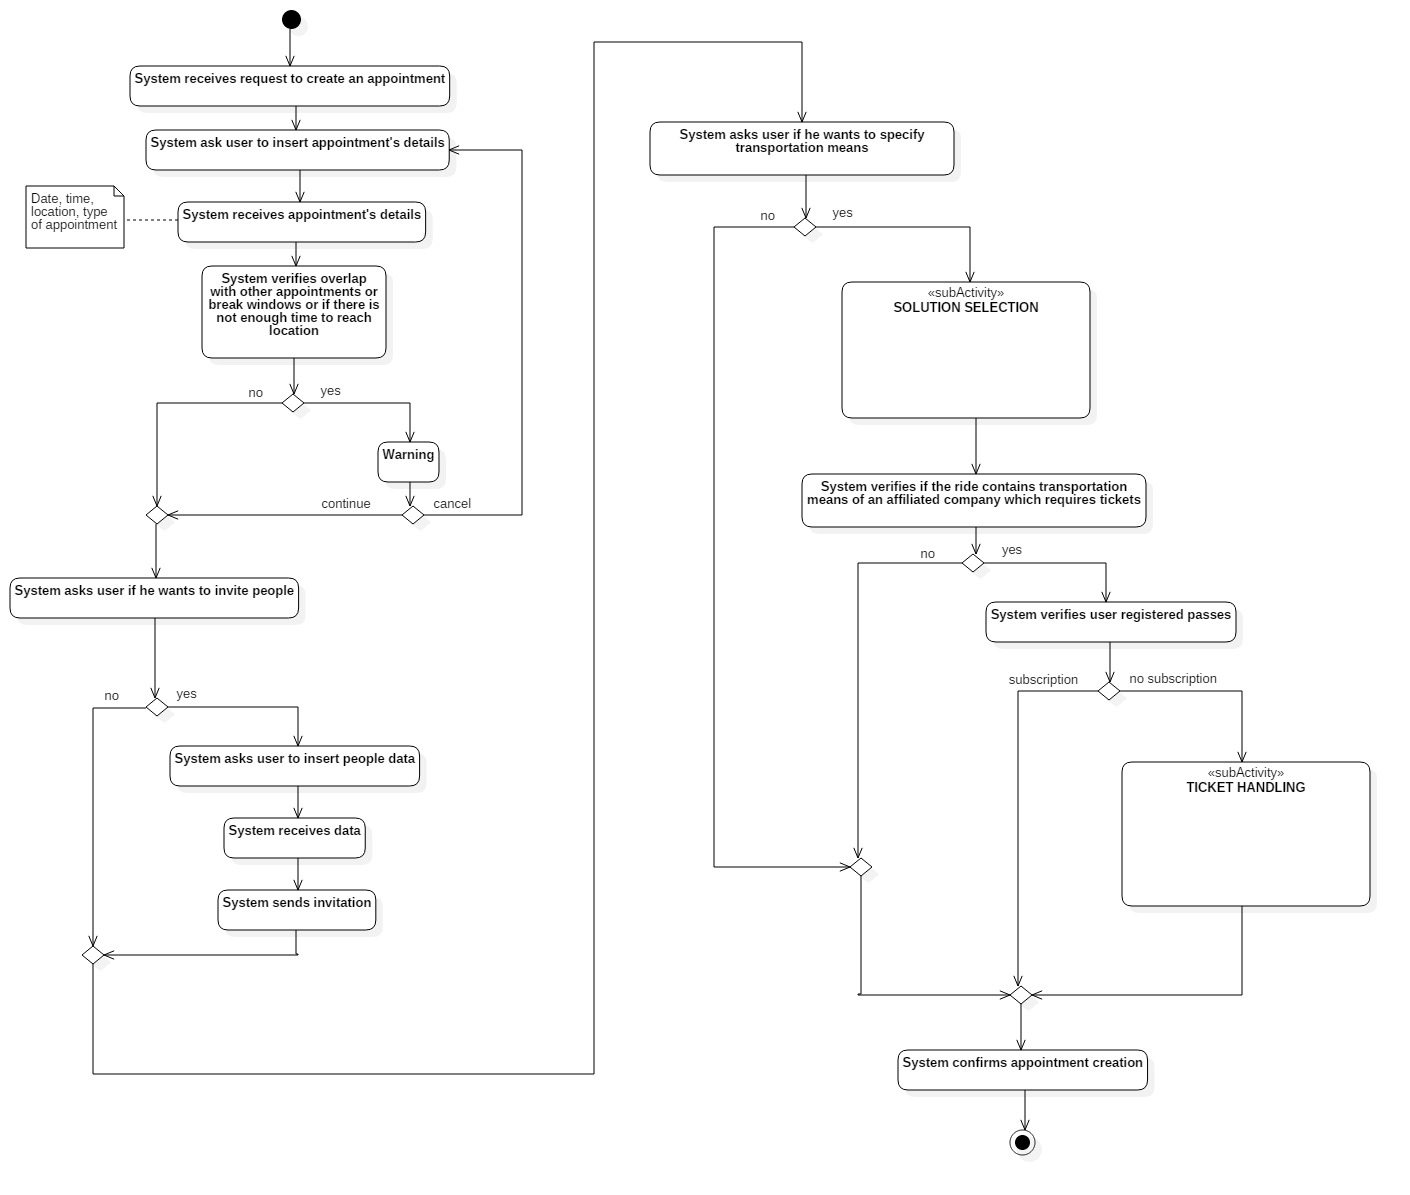
\includegraphics[width=\paperwidth-1]{Images/CreationAppointmentAD}}
			\caption{Creation appointment Activity Diagram}
		\end{figure}
		\begin{figure}[H]
			\centerline{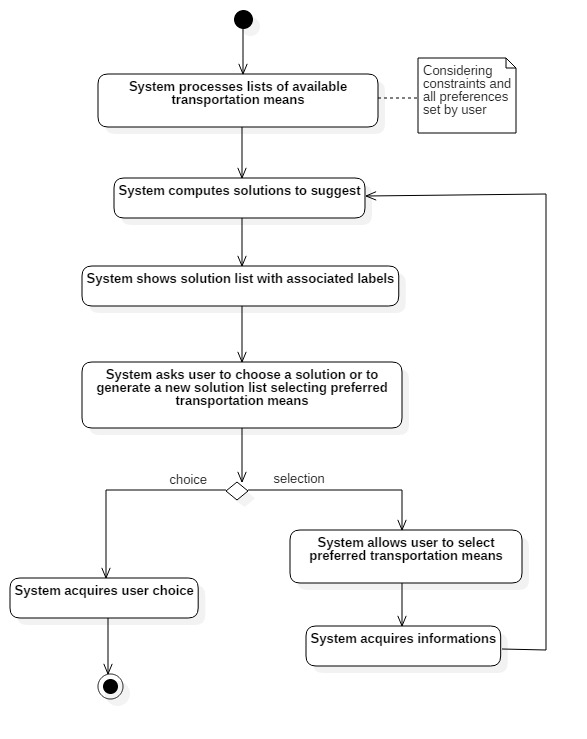
\includegraphics[height=0.35\paperheight]{Images/SolutionSelectionAD}}
			\caption{Solution selection Sub-Activity Diagram}
		\end{figure}
		\begin{figure}[H]
			\centerline{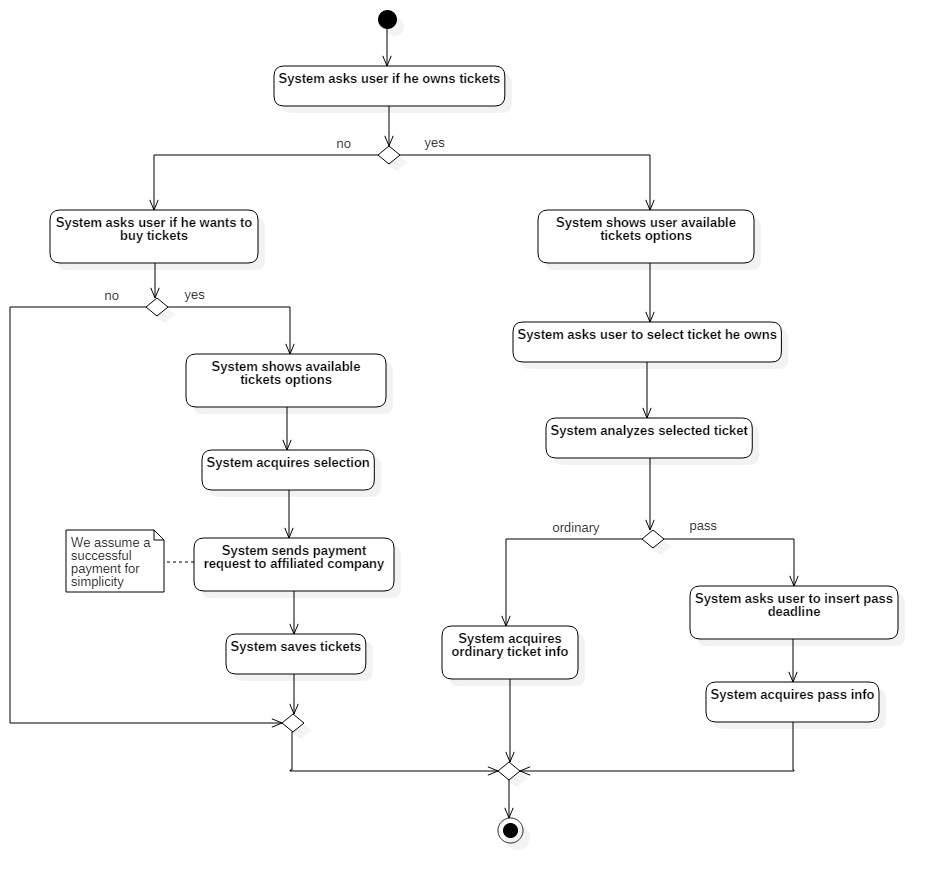
\includegraphics[height=0.35\paperheight]{Images/TicketHandlingAD}}
			\caption{Ticket handling Sub-Activity Diagram}
		\end{figure}
\subsection{Functional Requirements}
	\goal{G-become-registered}
	\begin{enumerate}[label={[R\arabic*]}]
		\item \mylabel{R-begin-registration}{the S2B must provide to every Person a way to begin the registration process}
		\item \mylabel{R-send-email}{after the insertion of the credentials and their \defined{validation}, the S2B has to send to the provided address an email with an activation link}
		\item \mylabel{R-unique-email}{the registration fails if the inserted email is already associated to an account}
		\item \mylabel{R-user-after-activation}{when the Person confirms through the activation link, he/she becomes a User}
		\item \mylabel{R-restart}{in the case of non \defined{valid credentials}, the system must reject them and restart the registration process}
		\item \mylabel{R-grant-access}{the S2B must grant access to the User if and only if the User inserts an existing email and the associated password}
	\end{enumerate}
	\begin{itemize}
		\item[] \myref{D-registration-proceed}
		\item[] \myref{D-email-always-received}
		\item[] \myref{D-everyone-email}
		\item[] \myref{D-user-remember}
		\item[] \myref{D-no-user-hacker}
	\end{itemize}

	\goal{G-pers-preferences}
	\begin{enumerate}[resume, label={[R\arabic*]}]
		\item \mylabel{R-change-preferences}{for each type of \defined{preference}, the S2B must provide the User the possibility to set or change the value(s)}
		\item \mylabel{R-store-preferences}{for each type of \defined{preference}, the S2B must store the preference value(s)}
	\end{enumerate}

	\goal{G-all-appointment}
	\begin{enumerate}[resume, label={[R\arabic*]}]
		\item \mylabel{R-new-appointment}{the system must provide a way to start the creation of a new appointment}
		\item \mylabel{R-appointment-details}{during the process the user shall insert the \defined{appointment details}}
	\end{enumerate}

	\goal{G-manage-agenda}
	\begin{enumerate}[resume, label={[R\arabic*]}]
		\item \mylabel{R-schedule-view}{existing appointments can be viewed together as a schedule view}
		\item \mylabel{R-daily-weekly}{the schedule can be daily or weekly}
		\item \mylabel{R-visualize}{from the schedule view, the system provides a way to visualize a single appointment and its details}
		\item \mylabel{R-edit-details}{after visualizing an appointment, the User who created it, can choose to edit its details}
		\item \mylabel{R-can-select}{in the schedule view the User can select one or more appointments}
		\item \mylabel{R-delete-selected}{in the schedule view, selected appointments can be deleted}	
	\end{enumerate}

	\goal{G-choose-sug}
	\begin{enumerate}[resume, label={[R\arabic*]}]
		\item \mylabel{R-solutions}{when time and location of the current appointment are set, the S2B produces a list of travel solutions with associated suggestions}
		\item \mylabel{R-choose-solution}{the S2B provide the user the possibility to choose one of the suggested travel solutions or leave the travel plan unspecified}
		\item \mylabel{R-select-preferred}{the S2B also provides the possibility to choose a preferred transportation mean}
		\item \mylabel{R-recompute-solutions}{when a new preferred transportation mean is selected the S2B has to recompute the list of solutions according to the new preference}
		\item \mylabel{R-bad-weather}{if weather forecast are bad: foot, bicycle motorbike are discouraged}
		\item \mylabel{R-strikes}{if strikes have been announced, public transport is discouraged}
		\item \mylabel{R-baggage-passengers}{in case of baggage or passengers a car is recommended}
		\item \mylabel{R-work}{in case of a work appointment, bicycle is discouraged}
	\end{enumerate}
	\begin{itemize}
	\item[] \myref{D-traffic}
    \end{itemize}
	
	\goal{G-invite}
	\begin{enumerate}[resume, label={[R\arabic*]}]
		\item \mylabel{R-can-invite}{when time and location of the current appointment are set, the S2B offers the possibility to invite other Users or Persons, through their emails}
		\item \mylabel{R-invite-send-email}{when a User or a Person is invited, the S2B will inform him/her sending an email}
	\end{enumerate}
	\begin{itemize}
		\item[] \myref{D-email-always-received}
	\end{itemize}
	
	\goal{G-owns-ticket}
	\begin{enumerate}[resume, label={[R\arabic*]}]
		\item \mylabel{R-accept-cc}{the S2B must accept credit card data from the User}
        \item \mylabel{R-check-cc}{the S2B must forward the credit card data to a credit institution to validate them}
		\item \mylabel{R-valid-cc}{the S2B must let the User use the credit card if and only if the inserted credit card data are valid}
		\item \mylabel{R-owns-ticket}{when the user selects a travel solution for which a ticket is expected, the S2B asks the User to specify if he/she owns a ticket (either ordinary or a pass, in which case the deadline has to be inserted)}
		\item \mylabel{R-buy-ticket}{if the user has selected a travel solution for which a ticket is expected and the User said to not own a ticket, the S2B asks him/her to buy a ticket (options available only for transportation means of \defined{affiliated companies})}
	\end{enumerate}
	
	\goal{G-locate}
	\begin{enumerate}[resume, label={[R\arabic*]}]
		\item \mylabel{R-provide-loc-service}{when a user visualizes an incoming appointment for which a shared vehicle of an affiliated company has to be used, the S2B provides a localization service}
	\end{enumerate}
	\begin{itemize}
		\item[] \myref{D-working-gps}
		\item[] \myref{D-provide-loc-API}
	\end{itemize}
	
	\goal{G-redirection}
	\begin{enumerate}[resume, label={[R\arabic*]}]
		\item \mylabel{R-rent-vehicle}{after the User has localized a vehicle, the S2B offers the possibility to rent it}
		\item \mylabel{R-redirects}{when the User selects the vehicle to rent, the app redirects him/her to the right company's app or site}
	\end{enumerate}

	\goal{G-notify}
	\begin{enumerate}[resume, label={[R\arabic*]}]
		\item \mylabel{R-incoming-notified}{when an appointment becomes incoming, the S2B sends a notification to the User}
		\item \mylabel{R-notChoosen-suggests}{if a travel plan has not already been set by the User, the notification suggests one}
		\item \mylabel{R-choosen-update}{if a travel plan has already been choosen but some complications (bad weather, traffic, strikes) have arosen the User is informed and a new feasible solution is suggested}
	\end{enumerate}
	
\subsection{Performance Requirements}
The system has to be able to respond to a possibly great number of simultaneous requests and
more generally to a great number of request throughout the day.
The S2B, at least for the start, will only be available for the Lombardy region. Based on demographic analysis (number of inhabitants, number of people under the age of 60, number of smartphones sold over the past 2 years), it was decided to design the S2B to support 100,000 users simultaneously, but scalability needs to be guaranteed.
\subsection{Design Constraints}
	\subsubsection{Standard compliance}
	To ensure interoperability the S2B will follow the W3C web standard and will be as adherent as possible to code practices in relation to the use of HTML/XHTML, CSS and Java programming language. Moreover, the use of non-opensource libraries will be avoided.
	\subsubsection{Hardware limitations}
		\begin{itemize}
		\item Mobile App: \newline
			* 3G connection\newline
			* GPS\newline
			* Space for app package
		\item Web App: \newline
			* Modern browser able to retrieve User's location
		\end{itemize}
	
	\subsubsection{Any other constraint}
\textbf{Regulatory policies}\newline
	The system will ask for users' payment informations and obviously, in addition to store them
	safely, will use them only for fees and rides payments.
	Moreover, the system will have to ask for users' permission in order to retrieve and use their
	positions.
	Email addresses will not be used for commercial uses.
\subsection{Software System Attributes} 
	\subsubsection{Reliability}
	The system must guarantee a 24/7 service. Very small deviations from this requirement will be
	obviously acceptable.
	\subsubsection{Availability}
	The S2B must guarantees a 3-nines availability (99.9 percent) with a downtime not greater than 8 hours per year.
	\subsubsection{Security}
User credentials and payment information will be stored. Data confidentiality is a primary concern.
In addition, when the user wants to buy tickets or rent a shared vehicle, the stored information must be sent to affiliated  transport Company systems or shared vehicle Company  systems. To ensure the security and the confidentiality of this information, the S2B must be able to adopt  access management protocols and communication protocols able to prevent not granted access and/or Sniffing/Spoofing activities performed by thirds.
	
	\subsubsection{Maintainability}
	The S2B must be designed in a way to easily correct defects or their cause,
	repair or replace faulty or worn-out components without having to replace still working parts,
	prevent unexpected working condition,
	maximize its useful life,
	maximize efficiency, reliability, and safety,
	meet new requirements,
	make future maintenance and
	cope with a changed environment.
	
	\subsubsection{Portability}
	The S2B must be able to run in all main mobile OS \textit{Android, iOS, Windows-Phone OS)} and to be supported by all the main Web Browser \textit{(Google Chrome, Safari, Firefox, Microsoft Edge)}.
	
